\documentclass[sigconf]{acmart}

\settopmatter{printacmref=true}

\fancyhead{}

\usepackage{balance}

\def\BibTeX{{\rm B\kern-.05em{\sc i\kern-.025em b}\kern-.08emT\kern-.1667em\lower.7ex\hbox{E}\kern-.125emX}}

\copyrightyear{2020}
\acmYear{2020}
\setcopyright{rightsretained}
\acmConference[SPAA '20]{Proceedings of the 32nd ACM Symposium on Parallelism in Algorithms and Architectures}{July 15--17, 2020}{Virtual Event, USA}
\acmBooktitle{Proceedings of the 32nd ACM Symposium on Parallelism in Algorithms and Architectures (SPAA '20), July 15--17, 2020, Virtual Event, USA}
\acmPrice{15.00}
\acmISBN{978-1-4503-6935-0/20/07}
\acmDOI{10.1145/3350755.3400234}
%\acmSubmissionID{123-A56-BU3}


\newcommand{\dec}{\operatorname{dec}}
\newcommand{\poly}{\operatorname{poly}}
\newcommand{\polylog}{\operatorname{polylog}}
\newcommand{\github}{\url{github.com/awestover/Parallel-Partition}}
\newcommand{\defn}[1]{{\textit{\textbf{\boldmath #1}}}}
\renewcommand{\paragraph}[1]{\vspace{0.09in}\noindent{\bf \boldmath #1.}} 
\usepackage{amsmath}
\usepackage{dsfont}
\def\E{\operatorname{\mathbb{E}}}
\usepackage{amssymb}
\usepackage{amsthm}

\newtheorem{thm}{Theorem}[section]
\newtheorem{lem}[thm]{Lemma}
\newtheorem{prop}[thm]{Proposition}
\newtheorem{clm}[thm]{Claim}
\newtheorem{cor}[thm]{Corollary}
\newtheorem{conj}[thm]{Conjecture}
\theoremstyle{remark}
\newtheorem{rem}[thm]{Remark}
\newtheorem{ex}[thm]{Example}

\newtheorem{theorem}{Theorem}[section]
\newtheorem{definition}[thm]{Definition}
\newtheorem{lemma}[thm]{Lemma}
\newtheorem{proposition}[thm]{Proposition}
\newtheorem{claim}[thm]{Claim}
\newtheorem{corollary}[thm]{Corollary}
\newtheorem{conjecture}[thm]{Conjecture}
\theoremstyle{remark}
\newtheorem{remark}[thm]{Remark}
\newtheorem{example}[thm]{Example}
\newtheorem{observation}[thm]{Observation}


\begin{document}

\fancyhead{}


\title{Brief Announcement \\In-Place Parallel-Partition Algorithms \\using Exclusive-Read-and-Write Memory}

\author{William Kuszmaul}
\authornote{Supported by a Hertz Fellowship, a NSF GRFP Fellowship, and NSF grant 1533644.}
\affiliation{%
  \institution{Massachusetts Institute of Technology}
}
\email{kuszmaul@mit.edu}

\author{Alek Westover}
\authornote{Supported by MIT PRIMES.}
\email{alek.westover@gmail.com}

\renewcommand{\shortauthors}{William Kuszmaul and Alek Westover}

\begin{abstract}
We present an in-place algorithm for the parallel-partition problem
with linear work and polylogarithmic span. The algorithm uses only
exclusive read/write shared variables and can be implemented using
parallel-for-loops without any additional concurrency considerations
(i.e., the algorithm is EREW). A key feature of the algorithm is that
it exhibits provably optimal cache behavior up to small-order factors.

We also present a second in-place EREW algorithm with work $O(n)$ and span
$O(\log n \cdot \log \log n)$, which is within an $O(\log\log n)$ factor of the
optimal span. By using this low-span algorithm as a subroutine within the
cache-friendly algorithm, we obtain a single EREW algorithm that combines their
theoretical guarantees: the algorithm achieves span $O(\log n \cdot \log \log
n)$ and exhibits optimal cache behavior. As an immediate consequence, we also
get an in-place EREW Quicksort algorithm with work $O(n \log n)$ and span
$O(\log^2 n \cdot \log \log n)$.

Whereas the standard EREW algorithm for parallel-partition is
memory-bandwidth bound on large numbers of cores, our cache-friendly
algorithm is able to achieve near-ideal scaling in practice by
avoiding the memory-bandwidth bottleneck. Our algorithm's performance
is comparable to that of the Blocked Strided Algorithm of Francis,
Pannan, Frias, and Petit, which is the previous state-of-the-art for
parallel EREW sorting algorithms, but which lacks theoretical
guarantees on its span and cache behavior.
\end{abstract}

\begin{CCSXML}
<ccs2012>
   <concept>
       <concept_id>10003752.10003809.10010170.10010171</concept_id>
       <concept_desc>Theory of computation~Shared memory algorithms</concept_desc>
       <concept_significance>500</concept_significance>
       </concept>
 </ccs2012>
\end{CCSXML}

\ccsdesc[500]{Theory of computation~Shared memory algorithms}

\keywords{Parallel Partition, EREW, in-place algorithms, cache-efficient}

\maketitle
\section{Introduction}

Given an array $A$ of length $n$ and a \defn{decider function} \\$\dec: A \to \{0, 1\}$
labelling the elements of $A$ as \defn{predecessors} (if $\dec(A[i])=0$) and
\defn{successors} (if $\dec(A[i])=1$), a \defn{partition} operation rearranges the
elements in an array so that predecessors occur before successors. In addition
to playing a central role in parallel Quicksort, the parallel-partition
operation is used as a primitive throughout parallel algorithms.\footnote{In
  several well-known textbooks and surveys on parallel algorithms
\cite{AcarBl16,Blelloch96}, for example, parallel partitions are implicitly
used extensively to perform what are referred to as \emph{filter} operations.}

A parallel algorithm can be measured by its \defn{work}, the time
needed to execute in serial, and its \defn{span}, the time to execute
on infinitely many processors. There is a well-known algorithm for
parallel partition on arrays of size $n$ with work $O(n)$ and span
$O(\log n)$ \cite{Blelloch96,AcarBl16}. Moreover, the algorithm uses
only exclusive read/write shared memory variables (i.e., it is an
\defn{EREW} algorithm).
This parallel-partition algorithm suffers from using a large amount of
auxiliary memory, however, and thus performs poorly in practice. 

\paragraph{Results}
We present an in-place EREW algorithm, that we call the \defn{Smoothed Striding
Algorithm}, for the parallel partition problem with work $O(n)$ and span
$\polylog(n)$ (Section \ref{sec:smoothing}). A key feature of this algorithm is
that it exhibits provably optimal cache behavior up to small-order factors.

We also present a second in-place EREW algorithm with work $O(n)$ and span
$O(\log n \cdot \log \log n)$, which is within an $O(\log\log n)$ factor of the
optimal span (Section \ref{sec:prefixbasedalg}). By using this low-span
algorithm as a subroutine within the Smoothed Striding algorithm, we are able to
obtain a single EREW algorithm that combines their theoretical guarantees: the
algorithm achieves span $O(\log n \cdot \log \log n)$ and optimal cache
behavior (Theorem \ref{thm:nicethm}). As an immediate consequence, we also get an in-place EREW Quicksort
algorithm with work $O(n \log n)$ and span $O(\log^2 n \cdot \log \log n)$.

Whereas the standard EREW algorithm for parallel partitioning is
memory-bandwidth bound on large numbers of cores, our cache-friendly
algorithm is able to achieve near-ideal scaling in practice by being in-place.
% by avoiding the memory-bandwidth bottleneck. 

The full analysis of the algorithms, along with the empirical evaluations are available in the extended paper \cite{ARXIV}.


\section{Preliminaries}\label{secprelim}

\paragraph{Workflow Model} We consider a simple language-based model of parallelism in which algorithms achieve parallelism through the use of \defn{parallel-for-loops} (see, e.g.,
\cite{Blelloch96,AcarBl16}); function calls within the inner loop
then allow for more complicated parallel structures (e.g., recursion). Our algorithms can also be implemented in the less restrictive PRAM model \cite{Blelloch96, AcarBl16}.

\paragraph{Memory Model}
Memory is \defn{exclusive-read} and \defn{exclusive-write} (i.e. we are in the
EREW model). That is, no two threads are ever permitted to attempt to read or
write to the same variable concurrently. Note that threads are not in lockstep
(i.e., they may progress at arbitrary different speeds), and thus the EREW
model requires algorithms to be data-race free in order to avoid the
possibility of non-exclusive data accesses.

In an \defn{in-place} algorithm, each thread is given $O(\polylog n)$
memory upon creation that is deallocated when the thread dies. This
memory can be shared with the thread's children. However, the depth of
the parent-child tree is not permitted to exceed $O(\polylog n)$.

\paragraph{Modeling Cache Misses}
We treat memory as consisting of fixed-size cache lines, each of some
size $b$. Each processor is assumed to have a small cache of
$\operatorname{polylog}{n}$ cache lines. A cache miss occurs on a
processor when the line being accessed is not currently in cache, in
which case some other line is evicted from cache to make room for the
new entry. Each cache is managed with the optimal off-line policy
(furthest-in-the-future).

% a LRU (Least Recently Used)
% eviction policy.

% However, we may assume for the sake of analysis that each cache is managed by
% the optimal off-line eviction strategy OPT (i.e. Furthest in the Future). This
% is because, up to resource augmentation, LRU eviction is $(1 + 1/\polylog
% n)$-competitive with OPT. Formally this is due to the following theorem by
% Sleator and Tarjan:
% \begin{theorem}[Resource Augmentation Theorem \cite{SleatorTa85}]
%   LRU operating on a cache of size $K\cdot M$ for some $K>1$ will incur at most
%   $1+\frac{1}{K-1}$ times the number of times cache misses of OPT operating on
%   a cache of size $M$, for the same series of memory accesses.
%   \label{thm:augmentation}
% \end{theorem}
% Because each processor's cache is managed by OPT (without loss of
% generality), we can assume that each processor \defn{pins} certain
% small arrays to cache (i.e., the elements of those arrays are never
% evicted).


\paragraph{The (Standard) Linear-Space Parallel Partition} The linear-space
implementation of parallel partition consists of two phases
\cite{Blelloch96,AcarBl16}:

\noindent\emph{The Parallel-Prefix Phase: }In this phase, the algorithm first
creates an array $D$ whose $i$-th element $D[i] = \dec(A[i])$ indicates whether
$A[i]$ is a predecessor ($\dec(A[i])=0$ if $A[i]$ is a predecessor and
$\dec(A[i]) = 1$ if $A[i]$ is a successor). Then the
algorithm constructs an array $S$ whose $i$-th element $S[i] = \sum_{j = 1}^i
D[i]$ is the number of predecessors in the first $i$ elements of $A$. The
transformation from $D$ to $S$ is called a \defn{parallel prefix sum} and can
be performed with $O(n)$ work and $O(\log n)$ span using a simple recursive
algorithm: (1) First construct an array $D'$ of size $n / 2$ with $D'[i] = D[2i
- 1] + D[2i]$; (2) Recursively construct a parallel prefix sum $S'$ of $D'$;
(3) Build $S$ by setting each $S[i] = S'[\lfloor i / 2 \rfloor] + A[i]$ for odd
$i$ and $S[i] = S'[i / 2]$ for even $i$. 

\noindent\emph{The Reordering Phase: }In this phase, the algorithm constructs
an output-array $C$ by placing each predecessor $A[i] \in A$ in position $S[i]$
of $C$. If there are $t$ predecessors in $A$, then the first $t$ elements of
$C$ will now contain those $t$ predecessors in the same order that they appear
in $A$. The algorithm then places each successor $A[i] \in A$ in position $t +
i - S[i]$. Since $i - S[i]$ is the number of successors in the first $i$
elements of $A$, this places the successors in $C$ in the same order that they
appear in $A$. Finally, the algorithm copies $C$ into $A$, completing the
parallel partition.

Both phases can be implemented with $O(n)$ work and $O(\log n)$
span. However, the algorithm uses multiple auxiliary arrays of size $n$.
Reducing the extra space below $o(n)$ has remained open until now, even when
the number of threads is fixed.

\section{An In-Place Partition Algorithm \\with Span $O(\log n \log \log
n)$}\label{sec:prefixbasedalg} We now outline the key algorithmic ideas needed
to make the classic Parallel Partition algorithm in-place with span $O(\log n
\log \log n)$. Although it is in-place, and hence more cache-efficient than the
standard out-of-place parallel partition algorithm, the algorithm described
here still exhibits poor cache behavior, and performs poorly in practice;
however, using this algorithm as a subroutine on a small subproblem in the
Smoothed Striding Algorithm will allow the Smoothed Striding Algorithm to
achieve span $O(\log n \log \log n)$ without sacrificing its good cache behavior.

\paragraph{Algorithm Outline}
Prior to beginning the algorithm, the first implicit step of the
algorithm is to count the number of predecessors in the array in
order to determine whether the majority of elements are either
predecessors or successors. We assume without loss of generality that the total
number of successors in $A$ exceeds the number of predecessors since otherwise
their roles can simply be swapped in the algorithm. Further, we assume for
simplicity that the elements of $A$ are distinct; this assumption can be removed.

Consider how to remove the auxiliary array $C$ from the Reordering
Phase. If one attempts to simply swap in parallel each predecessor
$A[i]$ with the element in position $j = S[i]$ of $A$, then the swaps
will almost certainly conflict. Indeed, $A[j]$ may also be a
predecessor that needs to be swapped with $A[S[j]]$. Continuing like
this, there may be an arbitrarily long list of dependencies on the
swaps.

To combat this, we begin the algorithm with a Preprocessing Phase in
which $A$ is rearranged so that every prefix is
\defn{successor-heavy}, meaning that for all $t$, the first $t$
elements contain at least $\frac{t}{4}$ successors. Then we compute
the prefix-sum array $S$, and begin the Reordering Phase. Using the
fact that the prefixes of $A$ are successor-heavy, the reordering can
now be performed in place as follows: (1) We begin by recursively
reordering the prefix $P$ of $A$ consisting of the first $4/5 \cdot n$
elements so that the predecessors appear before the successors; (2)
Then we simply swap each predecessor $A[i]$ in the final $1/5 \cdot n$
elements with the corresponding element $S[A[i]]$. The fact that the
prefix $P$ is successor-heavy ensures that, after step (1), the final 
$\frac{1}{5} \cdot n$ elements of (the reordered) $P$ are successors. 
This implies in step (2) that for each of the swaps between predecessors $A[i]$
in the final $1/5 \cdot n$ elements and earlier positions $S[A[i]]$, the latter
element will be in the prefix $P$. In other words, the swaps are now conflict
free.

Next, consider how to remove the array $S$ from the Parallel-Prefix
Phase. At face value, this would seem quite difficult since the
reordering phase relies heavily on $S$. Our solution is to
\emph{implicitly} store the value of every $O(\log n)$-th element of
$S$ in the ordering of the elements of $A$. That is, we break $A$ into
blocks of size $O(\log n)$, and use the order of the elements in each
block to encode an entry of $S$. (If the elements are not all
  distinct, then a slightly more sophisticated encoding is necessary.)
Moreover, we modify the algorithm for building $S$ to only construct
every $O(\log n)$-th element. The new parallel-prefix sum performs
$O(n / \log n)$ arithmetic operations on values that are implicitly
encoded in blocks; since each such operation requires $O(\log n)$
work, the total work remains linear.

Analysis of the algorithm yields the following theorem:
\begin{theorem}
  \label{thminplace}
  There exists an in-place algorithm using exclusive-read-write
  variables that performs parallel-partition with work $O(n)$ and span
  $O(\log n \cdot \log \log n)$.
\end{theorem}

\section{A Cache Efficient In-Place Parallel Partition Algorithm}\label{sec:smoothing}

\paragraph{The Strided Algorithm \cite{FrancisPa92}}
Our Smoothed Striding Algorithm borrows several structural ideas from a
previous algorithm of Francis and Pannan \cite{FrancisPa92}, which we call the
\defn{Strided Algorithm}\footnote{The original algorithm of Francis and Pannan
  \cite{FrancisPa92} does not consider the cache-line size $b$. Frias and Petit
later introduced the parameter $b$ \cite{Frias08} and showed that by setting
$b$ appropriately, one obtains an algorithm whose empirical performance is
close to the state-of-the-art.}. The Strided Algorithm is designed to behave
well on random arrays $A$, achieving span $\tilde{O}(n^{2/3})$ and exhibiting
only $n/b + \tilde{O}(n^{2/3} / b)$  cache misses on such inputs. On worst-case
inputs, however, the Strided Algorithm has span $\Omega(n)$ and incurs $n/b +
\Omega(n/b)$ cache misses. Our algorithm, the Smoothed Striding Algorithm,
builds on the Strided Algorithm by randomly perturbing the internal structure
of the Strided Algorithm; in doing so, we are able to provide provable
performance guarantees for arbitrary inputs and add a previously impossible
recursion step.
The original Strided Algorithm consists of two steps: \\
\emph{The Partial Partition Step.} 
Let $g \in \mathbb{N}$ be a
parameter, and assume for simplicity that $gb \mid n$. Partition the
array $A$ into $\frac{n}{gb}$ chunks $C_1, \ldots, C_{n / gb}$,
each consisting of $g$ cache lines of size $b$.
For $i \in \{1, 2, \ldots, g\}$, define 
$P_i$ to consist of the $i$-th cache line from each of the
chunks $C_1, \ldots, C_{n / gb}$. One can think of the $P_i$'s
as forming a strided partition of array $A$, since
consecutive cache lines in $P_i$ are always separated by a fixed
stride of $g - 1$ other cache lines.
The first step of the algorithm is to perform an in-place serial
partition on each of the $P_i$s, rearranging the elements within the
$P_i$ so that the predecessors come first. This step requires work
$\Theta(n)$ and span $\Theta(n/g)$.
\emph{The Serial Cleanup Step. }
For each $P_i$, define the \defn{splitting position} $v_i$ to be the position
in $A$ of the first successor in (the already partitioned) $P_i$. Define
$v_{\text{min}} = \min\{v_1, \ldots, v_{g}\}$ and define $v_{\text{max}} =
\max\{v_1, \ldots, v_{g}\}$. Then the second step of the algorithm is to
perform a serial partition on the sub-array $A[v_{\text{min}}],\ldots,
A[v_{\text{max}}-1]$. This completes the full partition of $A$.

\paragraph{The Smoothed Striding Algorithm}
To obtain an algorithm with provable guarantees for all inputs $A$, we
randomly perturb the internal structure of each of the $P_i$'s. Define
$U_1, \ldots, U_{g}$ (which play a role analogous to $P_1,
\ldots, P_g$ in the Strided Algorithm) so that each $U_i$ contains a
randomly selected cache line from each of $C_1, \ldots, C_{n /
  gb}$ (rather than containing the $i$-th cache line of each
$C_j$). This ensures that the number of predecessors in each $U_i$ is
a sum of independent random variables with values in $\{0, 1, \ldots,
n/g\}$.

By Hoeffding's Inequality, with high probability in $n$, the number of
predecessors in each $U_i$ is tightly concentrated around $\frac{\mu
  n}{g}$, where $\mu$ is the fraction of elements in $A$ that are
predecessors. It follows that, if we perform in-place partitions of
each $U_i$ in parallel, and then define $v_i$ to be the position in
$A$ of the first successor in (the already partitioned) $U_i$, then
the difference between $v_{\text{min}} = \min_i v_i$ and
$v_{\text{max}} = \max_i v_i$ will be small (regardless of the input array
$A$!).

Rather than partitioning $A[v_{\text{min}}],\ldots,
A[v_{\text{max}}-1]$ in serial, the Smoothed Striding Algorithm simply
recurses on the subarray. Such a recursion would not have been
productive for the original Strided Algorithm because the strided
partition $P_1', \ldots, P_g'$ used in the recursive subproblem would
satisfy $P_1' \subseteq P_1, \ldots, P_g' \subseteq P_g$ and thus each
$P_i'$ is already partitioned. That is, in the original Strided
Algorithm, the problem that we would recurse on is a worst-case input
for the algorithm in the sense that the partial partition step makes
no progress.


The main challenge in designing the Smoothed Striding Algorithm
becomes the construction of $U_1, \ldots, U_{g}$ without
violating the in-place nature of the algorithm. A natural approach
might be to store for each $U_i, C_j$ the index of the cache
line in $C_j$ that $U_i$ contains. This would require the storage of
$\Theta(n / b)$ numbers as metadata, however, preventing the algorithm
from being in-place. To save space, the key insight is to select a
random offset $X_j \in \{1, 2, \ldots, g\}$ within each $C_j$, and
then to assign the $(X_j + i \pmod g) + 1$-th cache line of $C_j$ to
$U_i$ for $i \in \{1, 2, \ldots, g\}$. This allows for us to construct
the $U_i$'s using only $O(n/(gb))$ machine words
storing the metadata $X_1, \ldots, X_{n / gb}$. By setting $g$ to
be relatively large, so that $\frac{n}{gb} \le
\operatorname{polylog}(n)$, we can obtain an in-place algorithm that
incurs $n (1 + o(1))$ cache misses.

The recursive structure of the Smoothed Striding Algorithm allows for
the algorithm to achieve polylogarithmic span. As an alternative to
recursing, one can also use the in-place algorithm from Section \ref{sec:prefixbasedalg}
 in order to partition the subarray. Doing so results in the following theorem:
\begin{theorem}
  \label{thm:nicethm}
  There exists an in-place EREW parallel-partition algorithm with
  work $O(n)$ that, with high probability in $n$, has span $O(\log n \log \log
  n)$ and incurs fewer than $(n+o(n))/b$ cache misses.
\end{theorem}

%   (since the
% algorithm from the Appendix has span only \\ $O(\log n \log \log
% n)$), while still incurring only $n (1 + o(1))$ cache misses (since
% the cache-inefficient algorithm from the Appendix is only used
% on a small subarray of $A$). We analyze both the recursive version of
% the Smoothed Striding Algorithm, and the version which uses as a final
% step the algorithm from the Appendix; one significant advantage
% of the recursive version is that it is simple to implement in
% practice.

% \paragraph{Formal Algorithm Description} Let $b < n$ be the size of a cache line, let $A$ be an input array of size
% $n$, and let $g$ be a parameter. (One should think of $g$ as being
% relatively large, satisfying $\frac{n}{bg} \le
% \operatorname{polylog}(n)$.)  We assume for simplicity that that $n$
% is divisible by $gb$, and we define $s = \frac{n}{gb}$.
% \footnote{This assumption can be made without loss of generality by treating $A$ as
% an array of size $n' = n + {(gb - n \pmod {gb})}$, and then treating
% the final $gb - n \pmod {gb}$ elements of the array as being
% successors (which consequently the algorithm needs not explicitly
% access). Note that the extra $n' - n$ elements are completely virtual, meaning they do not physically exist or reside in memory.
% }

% In the \defn{Partial Partition Step} the algorithm partitions the
% cache lines of $A$ into $g$ sets $U_1, \ldots, U_{g}$ of size
% $s = \frac{n}{gb}$ and then performs a serial partition on each $U_i$
% in parallel over the $U_i$'s. To determine the sets
% $U_1, \ldots, U_{g}$, the algorithm uses as metadata an array
% $X = X[1], \ldots, X[s]$, where each $X[i] \in \{1, \ldots,
% g\}$. 

% Formally, the Partial Partition Step performs the following procedure:
% \begin{itemize}
% \item Set each of $X[1], \ldots, X[s]$ to be uniformly random and
%   independently selected elements of $\{1, 2, \ldots, g\}$. For each $i \in
%   \{1, 2, \ldots, g\}$, $j \in \{1, 2, \ldots, s\}$, define
%   $$G_i(j) = (X[j] + i \pmod g) + (j - 1)g + 1.$$ Using this
%   terminology, we define each $U_i$ for $i \in \{1, \ldots, g\}$ to
%   contain the $G_i(j)$-th cache line of $A$ for each $j \in \{1, 2,
%   \ldots, s\}$. That is, $G_i(j)$ denotes the index of the $j$-th
%   cache line from array $A$ contained in $U_i$.

%   Note that, to compute the index of the $j$-th cache line in $U_i$,
%   one needs only the value of $X[j]$. Thus the only metadata needed by
%   the algorithm to determine $U_1, \ldots, U_g$ is the array
%   $X$. If $|X| = s = \frac{n}{gb} \le \operatorname{polylog}(n)$, then
%   the algorithm is in place.
  
% \item The algorithm performs an in-place (serial) partition on each
%   $U_i$ (and performs these partitions in parallel with one
%   another). In doing so, the algorithm, also collects
%   $v_{\text{min}}=\min_i{v_i}$, $v_{\text{max}}=\max_i{v_i}$, where
%   each $v_i$ with $i \in \{1, \ldots, g\}$ is defined to be the index
%   of the first successor in $A$ (or $n$ if no such successor
%   exists).\footnote{One can calculate $v_{\text{min}}$ and
%     $v_{\text{max}}$ without explicitly storing each of $v_1, \ldots,
%     v_{g}$ as follows. Rather than using a standard $g$-way parallel
%     for-loop to partition each of $U_1, \ldots, U_{g}$, one can
%     manually implement the parallel for-loop using a recursive
%     divide-and-conquer approach. Each recursive call in the
%     divide-and-conquer can then simply collect the maximum and minimum
%     $v_i$ for the $U_i$'s that are partitioned within that recursive
%     call. This adds $O(\log n)$ to the total span of the Partial
%     Partition Step, which does not affect the overall span
%     asymptotically. %% In practice, this can also be implemented using
%     %% CilkPlus Reducers (or OpenMP Reductions) \cite{FrigoLe09}, though
%     %% empirically we have found explicitly implementing the
%     %% divide-and-conquer structure to be worthwhile for performance.
%   }
  
%   The array $A$ is now partially partitioned, i.e. $A[i]$ is a
%   predecessor for all $i \le v_{\text{min}}$, and $A[i]$ is a successor
%   for all $i > v_{\text{max}}$.
% \end{itemize}

% The second step of the Smoothed Striding Algorithm is to complete the
% partitioning of $A[v_{\text{min}} + 1], \ldots, A[v_{\text{max}}]$. This can be done
% in one of two ways: The \defn{Recursive Smoothed Striding Algorithm}
% partitions $A[v_{\text{min}} + 1], \ldots, A[v_{\text{max}}]$ recursively using the
% same algorithm (and resorts to a serial base case when the subproblem
% is small enough that $g \le O(1)$); the \defn{Hybrid Smoothed Striding
%   Algorithm} partitions $A[v_{\text{min}} + 1], \ldots, A[v_{\text{max}}]$ using the
% in-place algorithm given in Theorem \ref{thminplace} with span $O(\log
% n \log \log n)$. In general, the Hybrid algorithm yields better
% theoretical guarantees on span than the recursive version; on the
% other hand, the recursive version has the advantage that it is
% simple to implement as fully in-place, and still achieves
% polylogarithmic span. 

% % Detailed pseudocode for the Recursive Smoothed Striding Algorithm can
% % be found in Appendix \ref{sec:pseudocode}.

% %% note: g > s should hold
% \paragraph{Algorithm Analysis} 
% We prove the following proposition regarding the Partial Partition Step of the
% Smoothed Striding Algorithm.
% \begin{proposition}
%   \label{prop:generalResult}
%   Let $\epsilon \in (0, 1/2)$ and $\delta \in (0, 1/2)$ such that
%   $\epsilon \ge \frac{1}{\poly(n)}$ and $\delta \ge
%   \frac{1}{\polylog(n)}$. Suppose $s > \frac{\ln
%     (n/\epsilon)}{\delta^2}$. Finally, suppose that each processor has
%   a cache of size at least $s + c$ for a sufficiently large constant
%   $c$.

%   Then the Partial-Partition Algorithm achieves work $O(n)$; achieves
%   span $O\paren*{b \cdot s}$; incurs $\frac{s+n}{b} + O(1)$ cache
%   misses; and guarantees with probability $1 - \epsilon$ that
%   $$v_{\text{max}}-v_{\text{min}} < 4 n \delta.$$
% \end{proposition}

% Using this we can analyze the hybrid and recursive smoothed striding algorithms.

% We will assume that both the hybrid and the recursive algorithms use $\epsilon
% = 1/n^c$ for $c$ of our choice (i.e. with high probability in $n$). Moreover,
% the Recursive Smoothed Striding Algorithm continues to use the same value of
% $\epsilon$ within recursive subproblems (i.e., the $\epsilon$ is chosen based
% on the size of the first subproblem in the recursion), so that the entire
% algorithm succeeds with high probability in $n$.

% For both algorithms, the choice of $\delta$ results in a tradeoff between cache
% misses and span. For the Recursive algorithm, we allow for $\delta$ to be
% chosen arbitrarily at the top level of recursion, and then fix $\delta  =
% \Theta(1)$ to be a sufficiently small constant at all levels of recursion after
% the first; this guarantees that we at least halve the size of the problem
% between recursive iterations\footnote{In general, setting $\delta = 1/8$ will
% result in the problem size being halved. However, this relies on the assumption
% that $gb \mid n$, which is only without loss of generality by allowing for the
% size of subproblems to be sometimes artificially increased by a small amount
% (i.e., a factor of $1 + gb / n = 1 + 1/s$). One can handle this issue by
% decreasing $\delta$ to, say, $1/16$.}. Optimizing $\delta$ further (after the
% first level of recursion) would only affect the number of undesired cache
% misses by a constant factor.

% Formally we prove the following performance results for these algorithms:
% \begin{corollary}
%   \label{cor:fullPartition}
% Suppose $b \le o(\log \log n)$. Then the Hybrid Smoothed Striding Algorithm using $\delta = \Theta\big(\sqrt{b/\log\log n}\big)$, achieves work $O(n)$, and with high probability in $n$, achieves span $O(\log n \log\log n)$ and incurs fewer than $(n+o(n))/b$ cache misses.\\\\
% \end{corollary}

% \begin{corollary}
%   \label{cor:groupedPartitionAlg}
%   With high probability in $n$, the Recursive Smoothed Striding Algorithm using parameter $\delta=1/\sqrt{\log n}$:
%   achieves work $O(n)$, attains span $O(b\log^2 n)$, and incurs $n/b \cdot (1 + O(1 / \sqrt{\log n}))$ cache misses. 
% \end{corollary}

% \section{Performance Comparisons}\label{secexp}
% \begin{figure}[h]
%   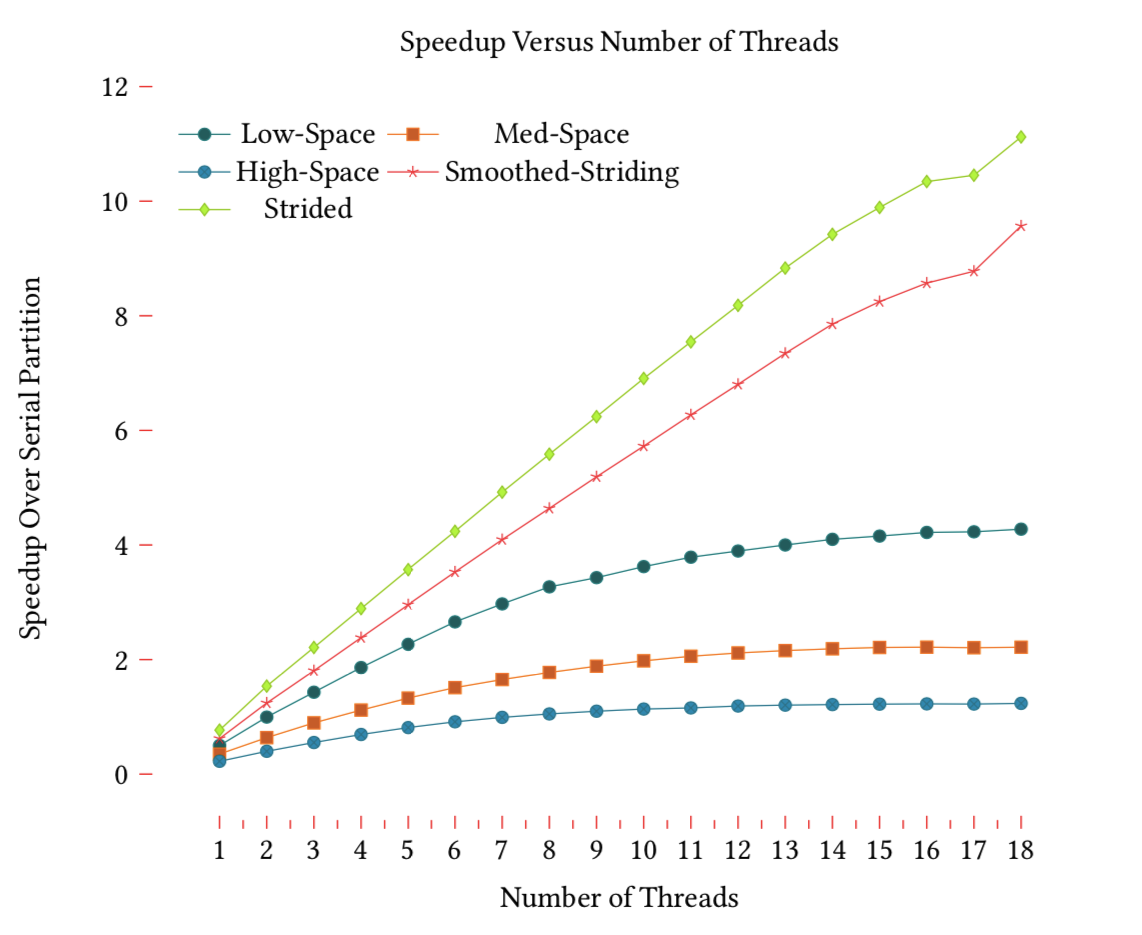
\includegraphics[width=\linewidth]{graph_performance.png}
% % \CILKtable 
% % \caption{We compare the performance of various partition implementations, relative to the Libc serial baseline, on random arrays of size $2^{30}$.
% %  The $x$-axis plots the number of worker threads being used, and the $y$-axis
% %  plots the multiplicative speedup over the serial baseline. Each time
% %  (including the serial baseline) is averaged over five trials.}
% %  \label{tablecilk}
% \end{figure}



\bibliographystyle{ACM-Reference-Format}
\bibliography{paper}

\end{document}




